% Setup - do not change
\documentclass[11pt]{article}
\usepackage[top=0.9in, left=0.9in, bottom=0.9in, right=0.9in]{geometry} 
\usepackage{parskip}

\usepackage[english]{babel}
\usepackage[utf8]{inputenc}
\usepackage{amsmath,amsthm,amssymb,graphicx,pdfpages,lipsum,hyperref}
\usepackage[none]{hyphenat}
\usepackage{csquotes}

\setlength\parindent{0pt}
%%%%%%%%%%%%%%%%%%%%%%%%%%%%%%%%%%%%%%%%%%%%%%%%%%%%%%%%%%%%%%%%%%%
% add other packages here if required
\usepackage{graphicx}
\usepackage{subcaption}

\usepackage[sorting = none]{biblatex}
\addbibresource{references.bib}

%%%%%%%%%%%%%%%%%%%%%%%%%%%%%%%%%%%%%%%%%%%%%%%%%%%%%%%%%%%%%%%%%%% the '%' symbol denotes comments

% Begin document creation
\title{\textbf{Predicting tip rate by crime count} \\ Creating Safety and travel patterns}
\author{
Insert Student Guoxuan Wang \\
Student ID: 1266123 \\
\href{https://github.com/MAST30034-Applied-Data-Science/mast30034-project-1-flgg0202.git}{report submission}
}

\begin{document}
\maketitle

\section{Introduction}
Crime rate is currently a pressing concern for every American. "This is a trend across the nation, drawing considerable attention from the public," the report states. According to a poll conducted by NewsNation Decision Desk HQ \cite{Crimepressing}, crime stands as the second most pressing issue for Americans, coming just after inflation. Being one of the prominent cities in the U.S., New York faces similar challenges. Under extensive media coverage, it seems that the city's crime rate has been on an upward trajectory in recent years. In an effort to provide both residents and tourists with safer travel routes, I aim to determine if there are any correlations between areas with higher crime rates and the utilization of TLC services, particularly during the late-night hours.

In this report, I will present two contrasting models and observe their performances on predicting tip rate around different regions in NYC and analyzing the impact of crime rates on the outcomes. Beyond benefiting taxi companies and drivers, I hope the findings of this study can also contribute to creating a safer urban environment.

Through the report, I analyze tip rate as well as the crime rate in different regions.I hope to provide insights that can assist New York's taxi drivers in pursuing higher earnings while ensuring their safety on the streets.

\subsection{Dataset}
The primary data source for this report is the "TLC Taxi Trip Record Data" published by the NYC Taxi \& Limousine Commission.\cite{tlc} This dataset includes, but is not limited to, attributes such as fare\_amount, tip\_amount, pick\_up\_location, etc. I have chosen to focus my analysis on yellow taxis. Yellow taxis are an iconic mode of transportation in New York City. They can be hailed on the streets or accessed at specific taxi stands. While they primarily operate in central Manhattan and other busy areas, they can transport passengers to any location within the city. The wide coverage of yellow taxis aids in providing a comprehensive analysis across different regions.

To ensure that the data remains unaffected by events like the COVID-19 pandemic and to analyze the most recent trends, I've selected data from the past six months, spanning from September 2022 to March 2023, as my dataset.

Furthermore, I've integrated some external data sources to enhance my analysis. These include "NYPD\_Complaint\_Data\_Current\_Year\_To\_Date"\cite{nypd} and "Borough Boundaries" \cite{boundary}from NYC Open Data. Additionally, the Crime map from arcgis.com\cite{map} has been used as a reference.
The "Borough Boundaries" provides delineations of New York's various administrative districts, enabling a clearer geographical view of data distribution. The "NYPD\_Complaint\_Data" offers detailed records of every crime reported in New York this year. Since it also contains the coordinates of where the crime took place, it is instrumental in assessing areas with potentially higher crime rates.
All these external data sources incorporate geographical aspects, aligning perfectly with the objectives of our study and meeting our expectations.




\section{Preprocessing}
After consolidating the yellow taxi data from September 2022 to March 2023, we obtained a total of 16,797,787 records. To ensure the data meets our criteria and to minimize memory usage, I adopted the following processing steps:

\subsection{Additional Feature Creation}

\begin{itemize} 
    \item To better study the variation in tips across different time frames, I introduced a feature named “time\_set”: data from 5 am to 12 pm is labeled as “Morning”, from 12 pm to 6 pm as “Afternoon”, from 6 pm to 11 pm as “Evening”, and from 11 pm to 5 am as “Late Night”.
\end{itemize} 

\begin{itemize} 
    \item To investigate the impact of trip duration on other features, I created “time\_duration\_minutes”: This calculates the difference between pickup and drop-off times to note the duration of each trip in minutes, offering insights into the length of the journey.
\end{itemize} 

\begin{itemize} 
    \item To analyze the effect of different travel speeds on other features, I introduced “average\_speed”. This is calculated by dividing “trip\_distance” by “time\_duration\_minutes”, determining the average speed of the vehicle during a particular journey.
\end{itemize}

\subsection{Data Wrangling}
\begin{itemize} 
    \item \textbf{Records with very short trip duration} were discarded; only data representing trips of 1km or longer were retained. Trips shorter than this were deemed insignificant and not representative of typical taxi journeys.
\end{itemize}

\begin{itemize} 
    \item \textbf{Only data entries with tips greater than 0 dollar} were preserved. As our primary focus is on tips, values below this threshold were deemed inconsistent with our research objectives.
\end{itemize}

\begin{itemize} 
    \item \textbf{Payments not of type 1} were retained. According to the Yellow Trip Data Dictionary, only type 1 payment methods result in tips. Data with tips under other categories are considered anomalies.
\end{itemize}

\begin{itemize} 
    \item \textbf{Fares greater than 3 dollar} were preserved. According to NYC regulations, the initial cost for a New York City taxi is \$3. Any fare data below this amount is seen as an outlier.
\end{itemize}


To better investigate the distribution of various features and consequently filter out inappropriate data, I utilized the plotting capabilities of Pandas.

Given the need for ample memory while working with Pandas and considering the extensive size of the original dataset, I sampled 5\$ of the data. The features I elected to visualize, due to their comprehensive representation, included: Trip Distance, Fare Amount, Average Speed, Time Duration, and Tip Amount. Through the generated boxplots, we identified outliers in each dataset. However, the overall data distribution was concentrated at lower values (refer to Figure 1a). Consequently, I computed the quantile for each feature, retaining only the data that fell within 1.5 IQR (see Figure 1b).

\begin{figure}[h]
    \centering
    
    \begin{subfigure}[b]{0.45\textwidth}
        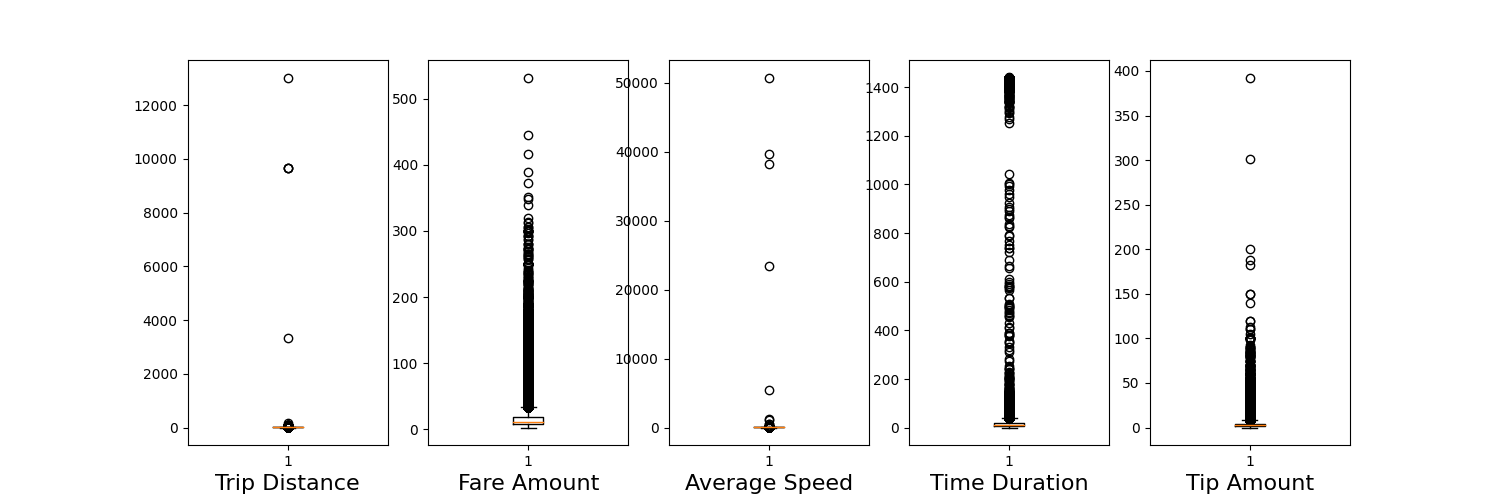
\includegraphics[width=\linewidth]{plots/first clean.png}
        \caption{first clean}
        \label{fig:figure1_sub1}
    \end{subfigure}
    \hfill 
    \begin{subfigure}[b]{0.45\textwidth}
        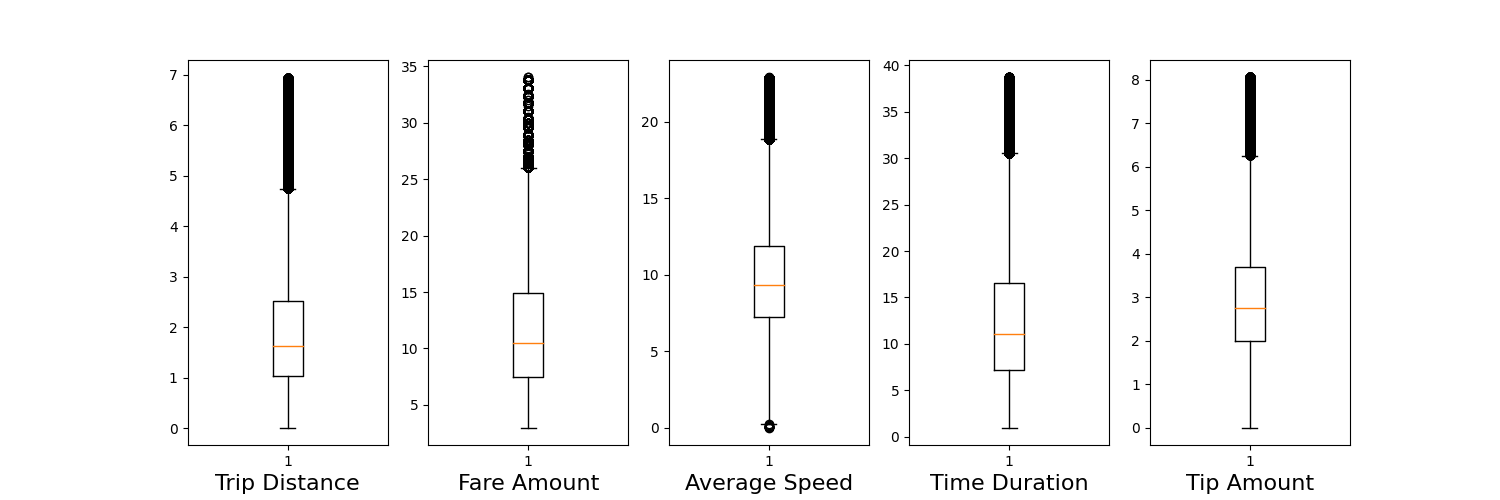
\includegraphics[width=\linewidth]{plots/second clean.png}
        \caption{second clean}
        \label{fig:figure2_sub2}
    \end{subfigure}
    
    \caption{Data cleaning}
    \label{fig:both_figures}
\end{figure}
Applying this same approach to the entire dataset, I was left with 13,058,002 records, approximately 78\% of the original dataset. Despite this refinement, the dataset still contained a plethora of entries irrelevant to my research objectives. Hence, for the data set that would ultimately train my model, I opted for a strategy where I grouped by PULocationID, computing averages for each respective zone. The resultant dataset for aggregation boasted the following features: 

\begin{itemize} 
    \item LocationID \quad\quad\quad •average tip  \quad\quad\quad•average fare
    \item tip rate (computed as average tip divided by average fare)\quad•average time
\end{itemize}


Regarding the NYPD data, the Borough Boundaries were provided in a JSON format, delineating geographical zones. I chose not to modify this file. As for the NYPD Complaint Data, since my study leans more towards the crime count in each zone rather than the specifics of the crime, I merely conducted NaN removal to ensure data reliability. From an initial count of 271,717 entries, I selected data from September 2022 to March 2023. Post NaN processing, I merged this with the data containing taxi zones. Ultimately, I grouped by LocationID, calculating the number of crimes corresponding to each location.

\subsection{Aggregation and Insights}

By plotting a pair plot using the sample, we discerned a conspicuous positive correlation between fare amount and tip amount. To further differentiate the profitability of each area, we introduced an additional feature named “Tip rate” prior to aggregation. This calculates the ratio of tip amount to fare amount for each region.

The final set of features retained for model training are: 
\begin{itemize} 
    \item LocationID \quad\quad\quad •average tip  \quad\quad\quad•average fare
    \item tip rate \quad\quad\quad\quad •average time \quad\quad\quad •crime count
    \item zone data inclusive of coordinates and borough information.
\end{itemize}



\section{Analysis and Geospatial Visualisation}
\subsection{Pre-merge Analysis}

From the pair plot(See Figure 2) of the TLC data, it was evident that there exists some level of positive correlation among fare, tip, and duration. Conversely, speed and duration appear to have a somewhat inverse relationship. These findings are consistent with our expectations when using taxis, with most data either following a normal distribution or being left-skewed. Yet, I observed that a significant portion of the tip amount data lies between \$0 and \$2. While there's some positive correlation of this distribution with other features, it largely appears random. Research indicates that taxi tips in New York typically range between 10\% and 20\% of the fare, and given the fare distribution, most fares are under \$20. Additionally, only tips made via credit cards are recorded; digital payment methods might prompt lower tip suggestions, such as \$1 to \$2. Considering these insights, I decided to identify more pronounced relationships with the tip from other features.
\begin{figure}[h]
    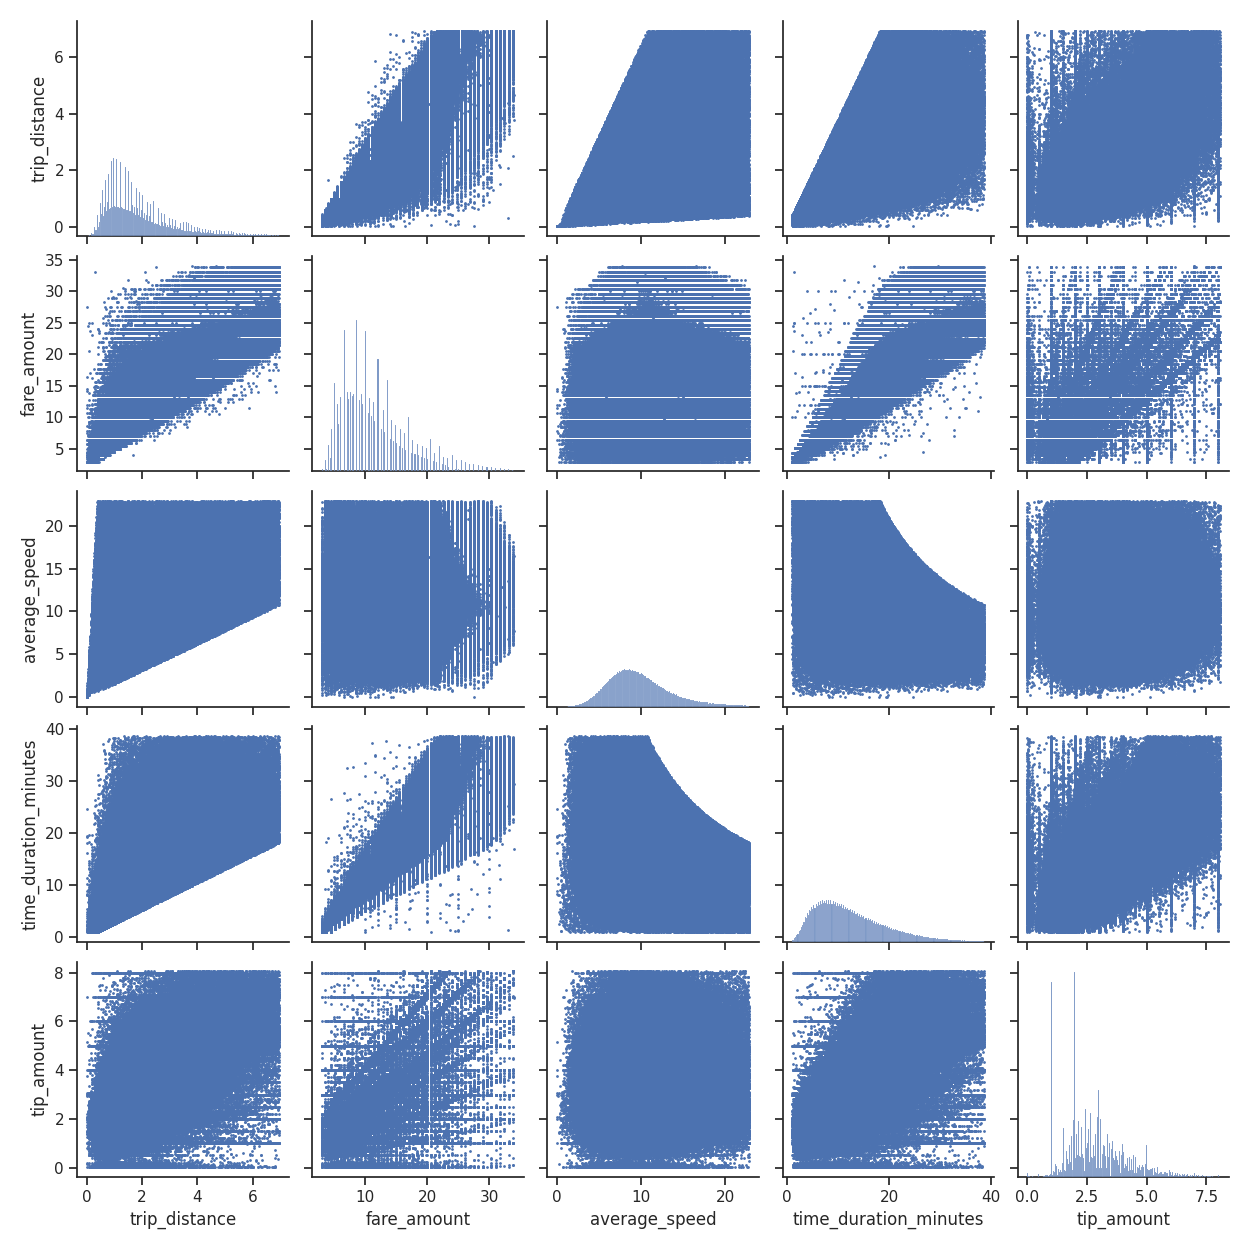
\includegraphics[width=0.6\textwidth]{plots/pair plot.png}
    \centering
    \caption{Pair plot}
\end{figure}


\subsection{Time Assumption}

\begin{figure}[h]
    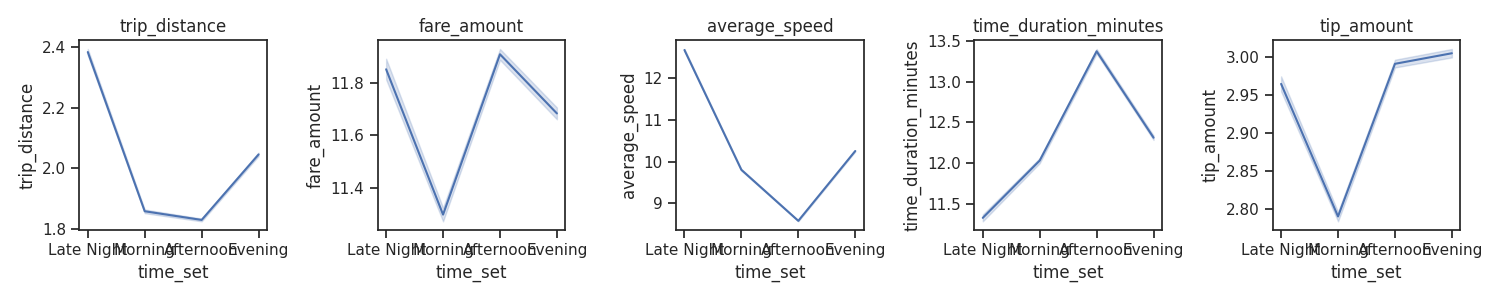
\includegraphics[width=0.9\textwidth]{plots/combined plot.png}
    \centering
    \caption{Time analysis}
\end{figure}

Crime rates can vary significantly based on the year, month, or even a specific day. For a broader logical exploration, I hypothesized that different times within a day might impact both crime rates and tips. Therefore, I categorized the data into morning, afternoon, evening, and late night. While visual representations did indicate some impact on tips based on these time segments, the magnitude of the variation was minimal, around \$0.2.(See Figure 3) This led me to believe that the time of day likely doesn't substantially influence tip distribution, and I ultimately chose not to factor it into my model training.


\subsection{Geographical Variations}

\begin{figure}[h]
    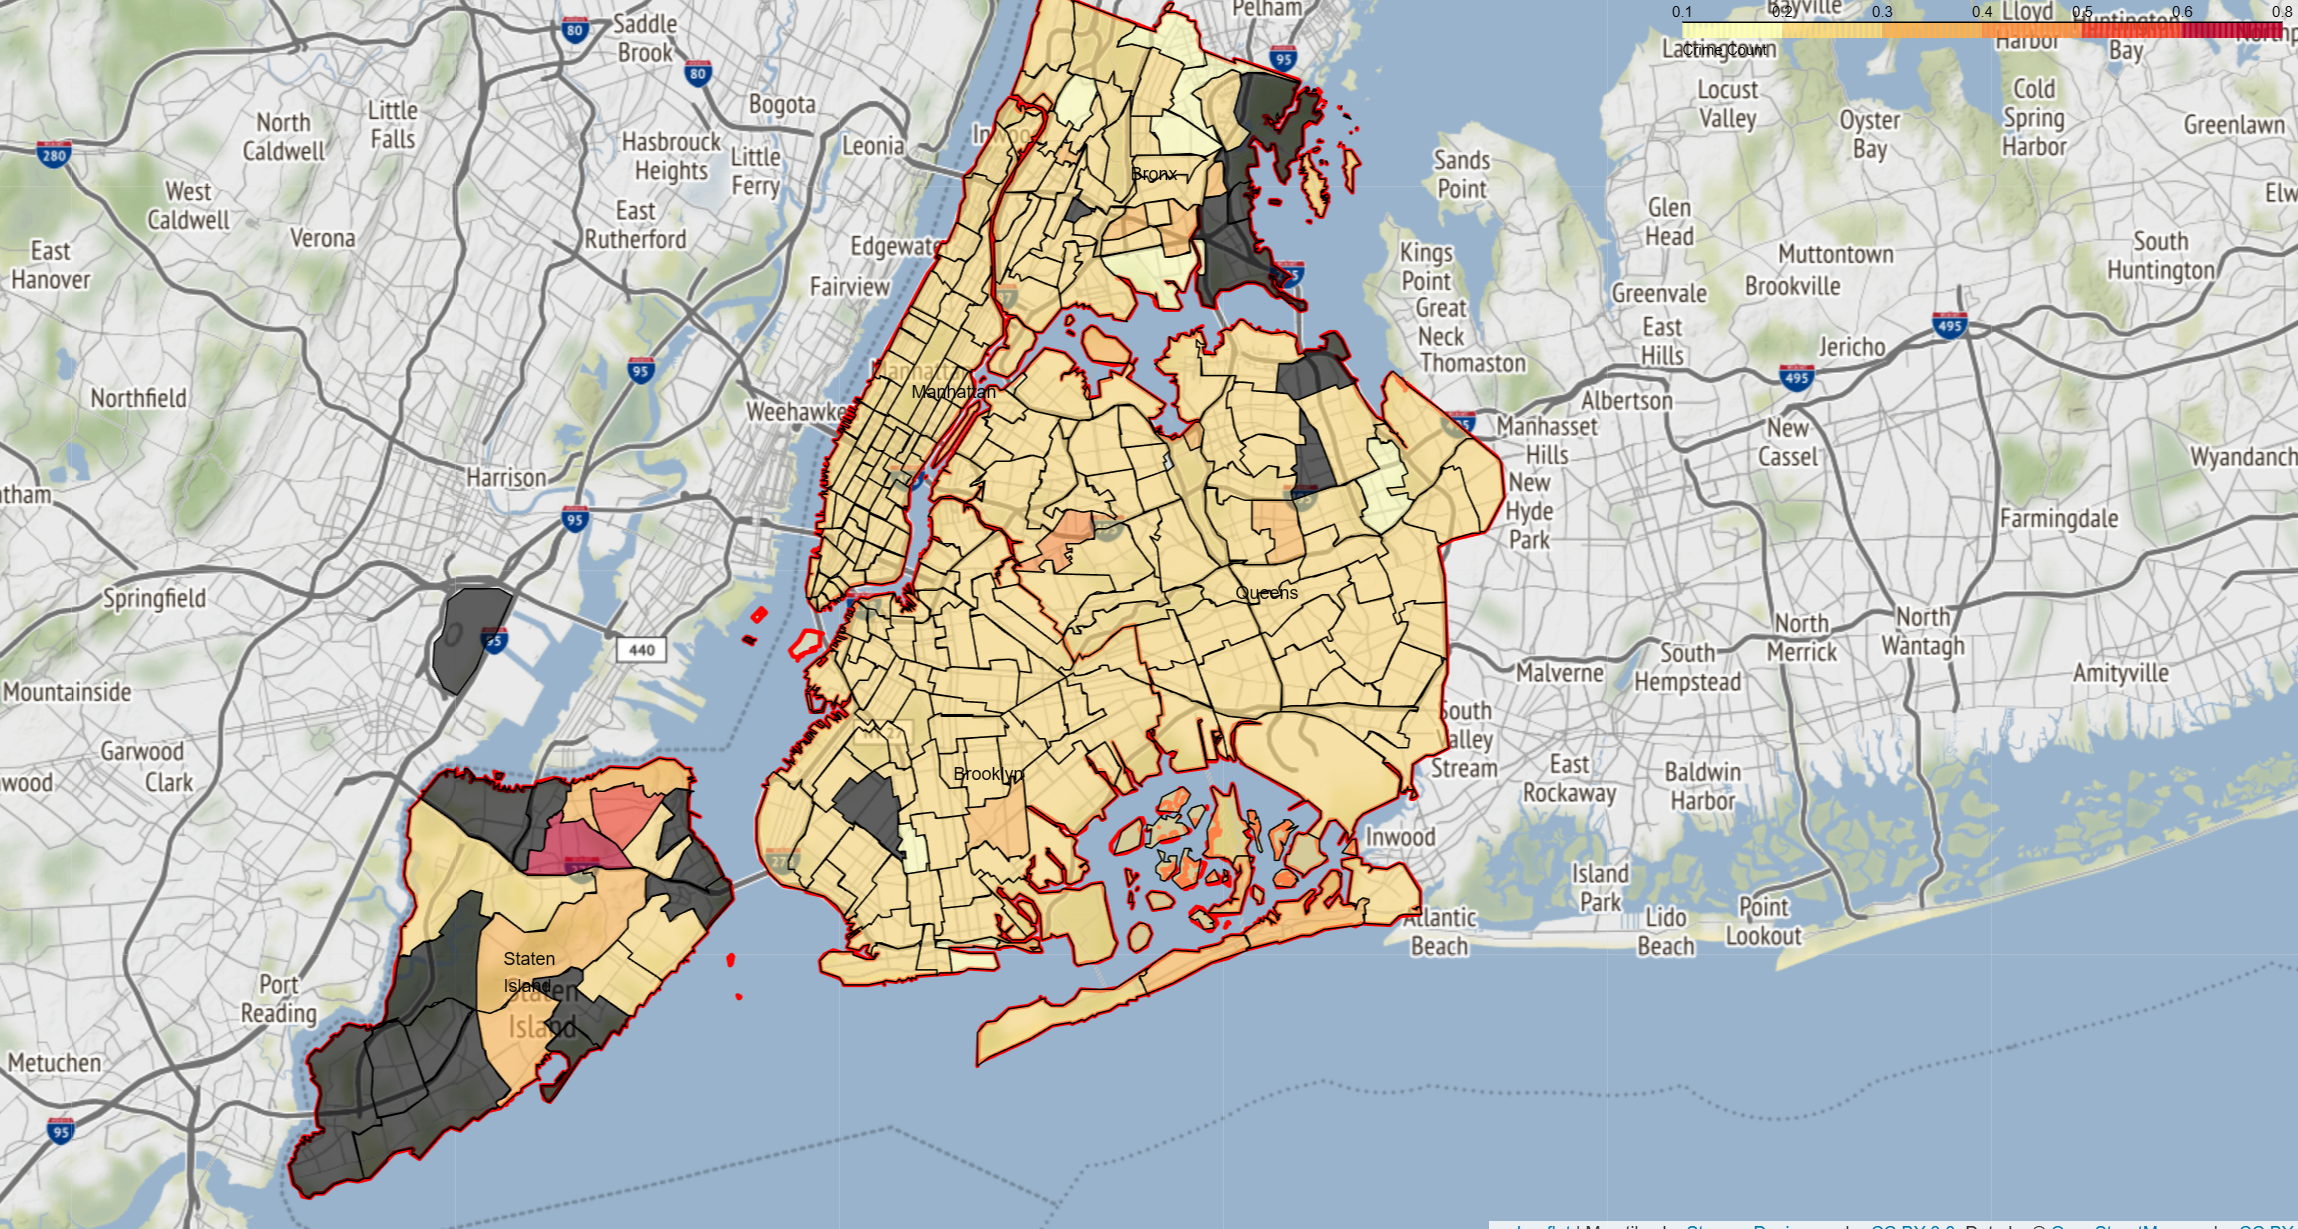
\includegraphics[width=0.7\textwidth]{plots/tip rate geo.png}
    \centering
    \caption{Tip rate geo}
\end{figure}

Utilizing geoPandas, I observed that the overall tip rate distribution across New York was relatively uniform(See Figure 4), predominantly between 0.1 and 0.3. However, Staten Island showcased a distinctly higher tip rate. Given that my previous analyses didn't reveal any pronounced relationship of the tip rate with other features, and considering that Staten Island represents a smaller fraction of the total data, I inferred this trend as a regional peculiarity.

\subsection{Crime Data}

\begin{figure}[h]
    \includegraphics[width=0.7\textwidth]{plots/crime count geo.png}
    \centering
    \caption{Crime Count geo}
\end{figure}
In terms of crime data, the distribution is more geographically distinct(See Figure 5). As illustrated, major administrative regions experience higher crime numbers. Queens, being a larger area, predominantly sees crime counts below 370, categorizing it as a relatively safer zone. Manhattan, Brooklyn, and the Bronx all have areas with higher crime numbers, often clustering around the boundaries between these boroughs. Staten Island, with the least amount of data, also exhibits the fewest crime figures, arguably making it the safest region.

Regrettably, there wasn't a clear correlation between crime amounts and tip rates. Given the even distribution of tip rates across various regions, leveraging crime counts to predict tip rates seems like an unavailable approach.


\section{Modelling}
\subsection{Random Forest Regression} Random Forest Regression is an ensemble algorithm that consists of numerous decision trees. Its prediction is based on the average outputs of all the individual trees. During the training phase, each decision tree is trained on a bootstrapped dataset. Thanks to its ensemble method, diversity, and robustness, Random Forest often delivers high accuracy, effectively avoids overfitting, and can handle a large number of nonlinear features. As our objective is to predict the tip rate, I believe Random Forest Regression is a suitable choice.\cite{rfr}

\subsection{Gradient Boosting} Gradient Boosting is a machine learning technique designed for both regression and classification problems. It optimizes the loss function by iteratively adding weak models, such as decision trees. In an effort to make the model more interpretable to taxi drivers, I've categorized the data into four distinct types, as indicated in the table below. Given that Gradient Boosting is widely used in business scenarios due to its outstanding performance, I'm convinced it's also a fitting choice for our project.\cite{gb}

The RFR model will be used initially to gauge the performance of the model, while the GB model will be employed for a more straightforward and intuitive classification prediction.

\section{Discussion}
\subsection{RFR}

\begin{table}[h]
\centering
\caption{RFR}
\label{table:example}
\begin{tabular}{|l|c|r|}
\hline
feature & importance & MSE \\
\hline
LocationID & 0.03930129 & 0.016239874170077485 \\
average time & 0.17301377 &  \\
crime count & 0.04445915 &  \\
average fare & 0.30969455 &  \\
average tip & 0.43353124 &  \\
\hline
\end{tabular}
\end{table}

\begin{figure}[h]
    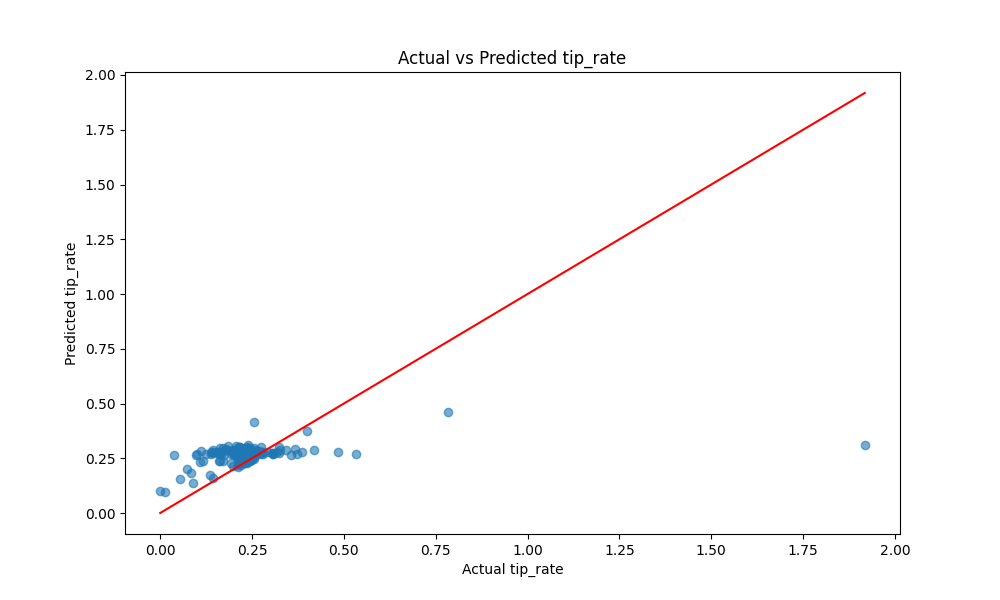
\includegraphics[width=0.7\textwidth]{plots/RF result.png}
    \centering
    \caption{RF} 
\end{figure}
To evaluate the model, I employed the Mean Squared Error (MSE). MSE provides an intuitive understanding of the magnitude of model errors. A lower MSE typically indicates better model performance. Additionally, I utilized feature importance to gauge the significance of each feature. As shown in Table 1, the model's MSE is 0.0162398741, suggesting that our model has a commendable predictive capacity. From Figure 6, it's evident that our model's predictions align closely with the actual values. Nevertheless, a glance at t1 reveals that both 'LocationID' and 'crime count' have rather low importance, implying that there seems to be no significant correlation between tip rate, location, and crime count.


\subsection{GB}

\begin{figure}[h]
    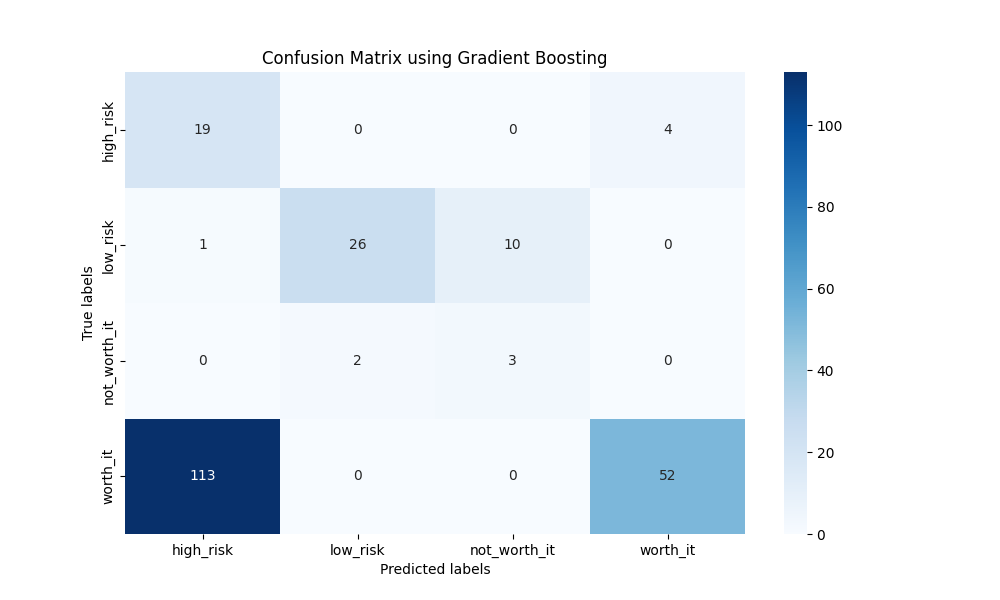
\includegraphics[width=0.7\textwidth]{plots/GB heat map.png}
    \centering
    \caption{GB heat map} 
\end{figure}

\begin{table}[h]
\centering
\caption{GB}
\label{table:example}
\begin{tabular}{|l|c|c|r|}
\hline
label & precision & recall & f1-score\\
\hline
high risk & 0.14 & 0.83 & 0.24\\
low risk & 0.93 & 0.70 & 0.80\\
not worth & 0.23 & 0.60 & 0.33\\
worth it & 0.93 & 0.32 & 0.47\\
\hline
\end{tabular}
\end{table}

As presented in the Table 2, the GB model does not exhibit stellar performance, with an accuracy of merely 0.43478. It accurately predicts low-risk areas, but its predictions for high-risk and not worth areas leave much to be desired. While the overall prediction for 'worth it' is not up to the mark, it still boasts high precision. Through Figure 7, we discern that the model predicts the 'worth it' areas with a high degree of accuracy. However, it seems the model mistakenly classifies a considerable portion of 'worth it' data as 'high risk'. I surmise this misclassification stems from the vast distributional differences between the 'tip rate' and 'crime count' features. Nonetheless, given the model's accuracy in determining 'worth it' areas, it remains valuable as a reference.
\section{Recommendations}
From the performance of the two models and our research into the data, we find that the majority of tip rates tend to cluster at lower values. Given the skewed distribution of crime counts, it's unrealistic to predict and suggest a location that offers both safety and high earnings.

Meanwhile,since the tip rate doesn't notably shift due to varying crime counts, I recommend taxi drivers to avoid areas with high crime rates, such as the boundary between Brooklyn and Queens, as well as the interface of Manhattan and the Bronx. Prioritizing personal safety is paramount. If areas with high crime rates neither enhance nor ensure consistent earnings, it is prudent to steer clear of those areas.

However, as noted in Section 3, Staten Island boasts generally higher tip rates coupled with an exceptionally low crime rate. This trend could be attributed to its relatively smaller size and less mature public transportation system, making the taxi service more sought-after. Yet, upon studying locations in Staten Island, I observed that most are tourist attractions and are considerably distanced from the main city. Therefore, spending a substantial amount of time daily in this region isn't advisable. Nonetheless, I strongly recommend drivers to allocate a portion of their mornings or afternoons to serve Staten Island. Doing so might not only sidestep the rush hours but also promise substantial earnings.
\section{Conclusion}
In this report, we sought to identify regions in New York where taxi drivers can earn the highest income while ensuring their safety. By analyzing data from two models, we cannot definitively link crime counts to tip rates. However, areas like Staten Island, which are both safe and lucrative, are undoubtedly worthy of consideration by drivers. Our research also suggests that recklessly venturing into high-crime areas is unwise, and drivers should prioritize their safety above all.

Through this investigation, I urge the government to pay serious attention to the rising crime rates and address the root causes. I firmly believe that with further research into more samples in the future, we can build a safer and more prosperous metropolis.
\clearpage


% BEGIN REFERENCES SECTION
\printbibliography

\end{document}